\documentclass{beamer}

\usepackage{svg}

\usetheme{Boadilla}
\usecolortheme{dolphin}
\setbeamertemplate{navigation symbols}{}
\setbeamertemplate{sections/subsections in toc}[sections numbered]

\setbeameroption{hide notes}
% \setbeameroption{show only notes}
% \setbeameroption{show notes on second screen=right}

\title[Embedded Trace]
{Embedded Trace: Assessing Data Dependence and Age}
\author[]{Hossein Afkar}
\institute{DRTS Lab}
\date{\today}

\begin{document}

\setbeamertemplate{footnote}{%
  \parindent 1em\noindent%
  \raggedright
  \insertfootnotetext\par%
}

\frame{\titlepage}

\begin{frame}
    \frametitle{Outline}
    \tableofcontents[hideallsubsections]
\end{frame}

\AtBeginSection[]
{
    \begin{frame}{Outline}
        \tableofcontents[currentsection]
    \end{frame}
}

\section{Preface}
\begin{frame}
    \frametitle{Preface}
    \begin{itemize}
        \item ETM trace evolution and examples.
        \item Data Age and Cause-Effect Chains.
        \item Online Assessment Timely Progress
    \end{itemize}
\end{frame}
\section{ETM: Trace Evolution}
\begin{frame}
    \frametitle{ETM Progression in Time}
    \begin{itemize}
        \item Advanced architectural improvements have found their way
            into the embedded systems. ETM also needed to evolve with these
            improvements and features.
        \item ETMv1 started with ARM7TDMI. An architecture without speculation
            and a simple three stage pipeline.
        \item ETMv4 is present in ARMv8.x which is a speculating machine with
            a more advanced pipeline.
        \item Therefore ETM needs to provide different information with
            different iteration of the hardware.
    \end{itemize}
    \footnotetext{Preußer, Thomas B., et al. "Everything You Always Wanted to Know About Embedded Trace." Computer 55.2 (2022): 34-43.}
\end{frame}
\begin{frame}
    \frametitle{ETMv1: Providing View Into the Pipeline}
    \begin{itemize}
        \item ETMv1 provides a view into the core via the execution stage of
            the pipeline.
        \item Every Instruction is cycle counted regardless.
    \end{itemize}
    \begin{figure}
        \centering
        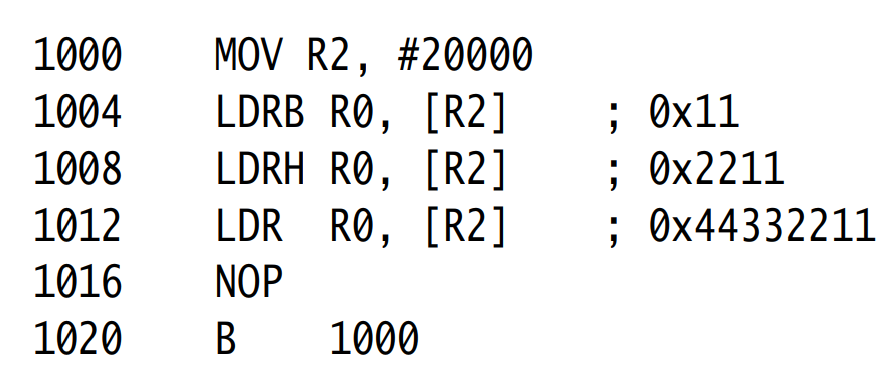
\includegraphics[width=0.80\columnwidth]{etmv11.png}
        \caption{Sample Traced Code}
        \label{fig:ETMv11}
    \end{figure}
\end{frame}
\begin{frame}
    \frametitle{ETMv1: Sample Trace} 
    \begin{figure}
        \centering
        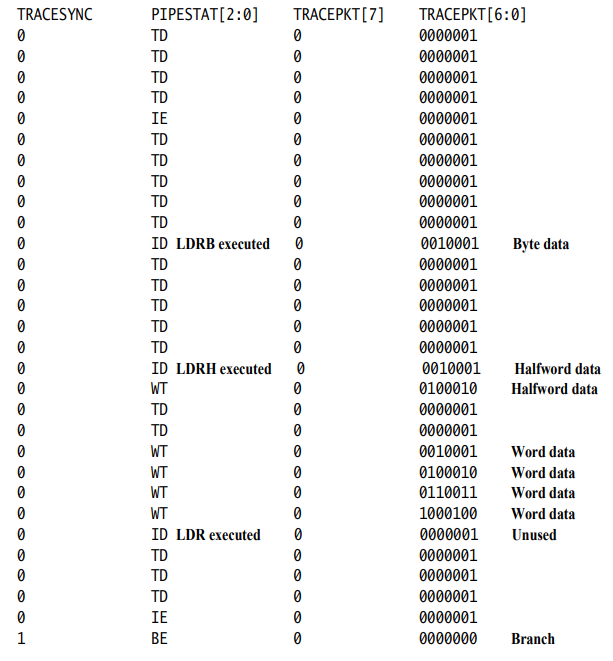
\includegraphics[width=0.55\columnwidth]{etmv12.png}
        \caption{Sample Traced Code}
        \label{fig:ETMv12}
    \end{figure}
\end{frame}
\begin{frame}
    \frametitle{ETMv4: Changing The View}
    \begin{itemize}
        \item For advanced architectures a view into the pipeline was no longer
            sufficient.
        \item To statisfy the needs of a speculating cpu core ETMv4
            specification is designed.
        \item Cycle counting is only possible when instructions batches are
            commited (This happens at branch boundaries and with enough
            configuration on Loads and Stores).
        \item So we can measure basic blocks easily in speculative processors.
    \end{itemize}
\end{frame}
\begin{frame}
    \frametitle{ETMv4: Sample Trace} 
        \begin{figure}
        \centering
        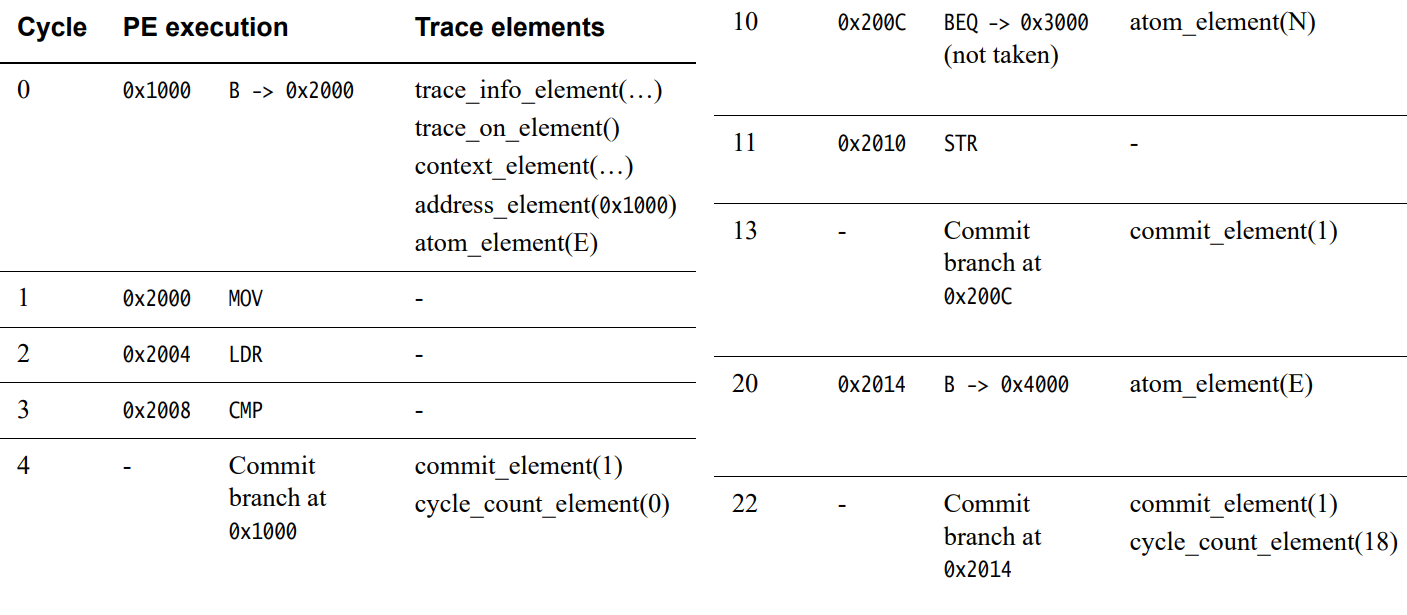
\includegraphics[width=0.90\columnwidth]{etmv4.png}
        \caption{Sample Traced Code}
        \label{fig:ETMv4}
    \end{figure}
\end{frame}
\section{Data Age and Cause-Effect Chains}
\begin{frame}
    \frametitle{Synthesizing Job-Level Dependencies for Automotive
    Multi-Rate Effect Chains}
    \begin{itemize}
        \item Real-time systems require a formal guarantee of
            timing-constraints, not only for individual tasks but also
            for data-propagation.
        \item Meeting timing constraints is difficult with multi-rate tasks
            chains in which tasks are activated with different periods.
        \item Data age constraints are commonly found in the control systems.
        \item It is important to know how long input data affects an output.
    \end{itemize}
    \footnotetext{Schlatow, Johannes, et al.
    "Data-age analysis and optimisation for cause-effect chains in automotive
    control systems." 2018 IEEE 13th international symposium on industrial
    embedded systems (SIES). IEEE, 2018.}
\end{frame}
\begin{frame}
    \frametitle{Cause-Effect Chain}
    \begin{itemize}
        \item Cause-Effect chain is denoted by $\psi = (\tau_i, \tau_{i+1}, \tau_{i+2}, ...)$
        \item Which corresponds to alternating read and write events $(r_i, w_i, r_{i+1}, w_{i+2}, r_{i+2}, ...)$
        \item $\tau_{i+1}$ reads data from $\tau_{i}$ and writes data for $\tau_{i+2}$.
        \item Data age describes the maximum age of the input data on which an
            output is based of.
    \end{itemize}
\end{frame}
\begin{frame}
    \frametitle{Task Model}
    \begin{figure}
        \centering
        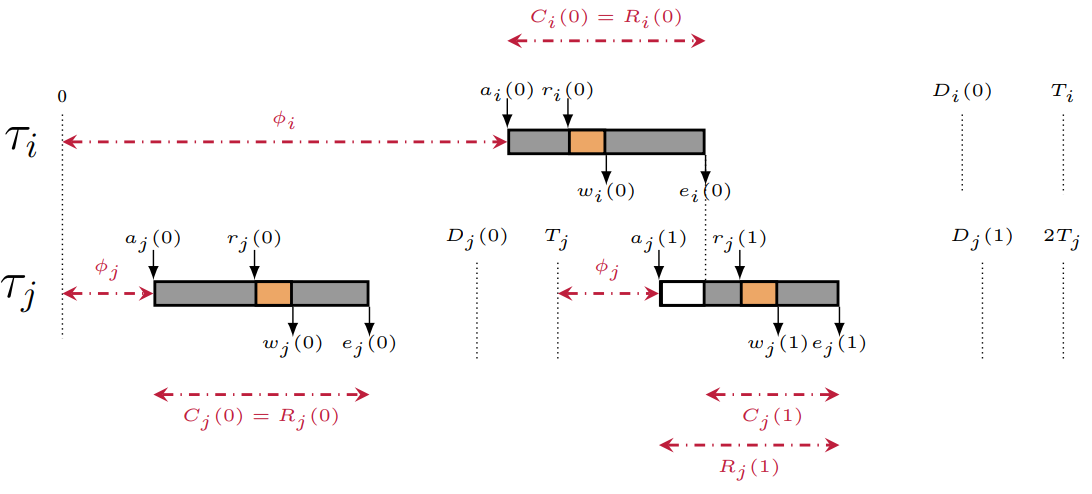
\includegraphics[width=0.95\columnwidth]{tm.png}
        \caption{Task Model Proposed by the Paper}
        \label{fig:tm}
    \end{figure}
\end{frame}
\begin{frame}
    \frametitle{Data Flow in Automotive Tasks}
    \begin{itemize}
        \item In the automotive industry, three paradigms (explicit, implicit
            and LET communication) are typically applied
            \begin{itemize}
                \item Explicit Communications: Shared Registers Access.
                \item Implicit Communications: Tasks have their input values
                    before the execution starts. And output is written at
                    the end of the task in a shared register.
                \item Logical Execution Time (LET): In this model,
                    the input values of a task are always read at the release
                    of the task. The output values become available once the
                    next period starts. 
            \end{itemize}
            \footnotetext{Becker, Matthias, et al. "End-to-end timing analysis
            of cause-effect chains in automotive embedded systems."
            Journal of Systems Architecture 80 (2017): 104-113.}
    \end{itemize}
\end{frame}
\begin{frame}
    \frametitle{Explicit Communication}
    \begin{figure}
        \centering
        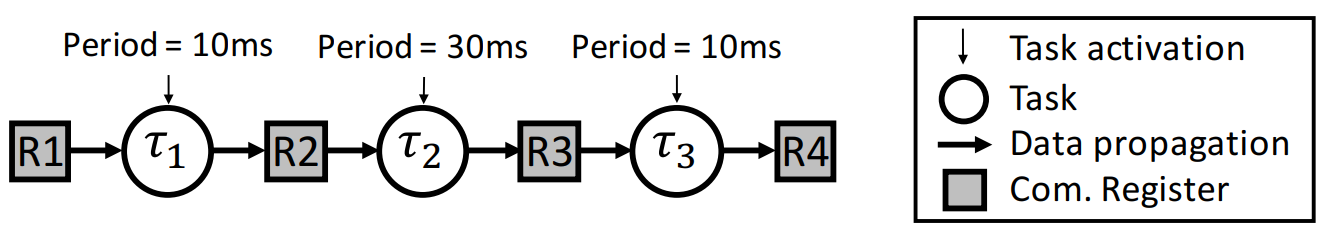
\includegraphics[width=1.0\columnwidth]{task.png}
        \caption{Register communication among communicating tasks}
        \label{fig:task}
    \end{figure}
    \footnotetext{Becker, Matthias, et al. "Synthesizing job-level dependencies
    for automotive multi-rate effect chains." 2016 IEEE 22nd International
    Conference on Embedded and Real-Time Computing Systems and Applications
    (RTCSA). IEEE, 2016.}
\end{frame}
\begin{frame}
    \frametitle{Data Dependency Graph}
    \begin{itemize}
        \item Data dependency graph is used in compilers to perform
            optimizations and reorderings.
        \item LLVM uses data dependency graph to track loop level dependencies
        \item Data dependecy graph can be constructed using AST or an IR (or Binary IL).
        \item Finding a path from a data read node can lead us to its
            propagation inside a program.
    \end{itemize}
    \footnotetext{D. J. Kuck, R. H. Kuhn, D. A. Padua, B. Leasure, and M. Wolfe
    (1981). DEPENDENCE GRAPHS AND COMPILER OPTIMIZATIONS.}
\end{frame}
\begin{frame}
    \frametitle{Example of Data Depnedecy Graph}
    \begin{figure}
        \centering
        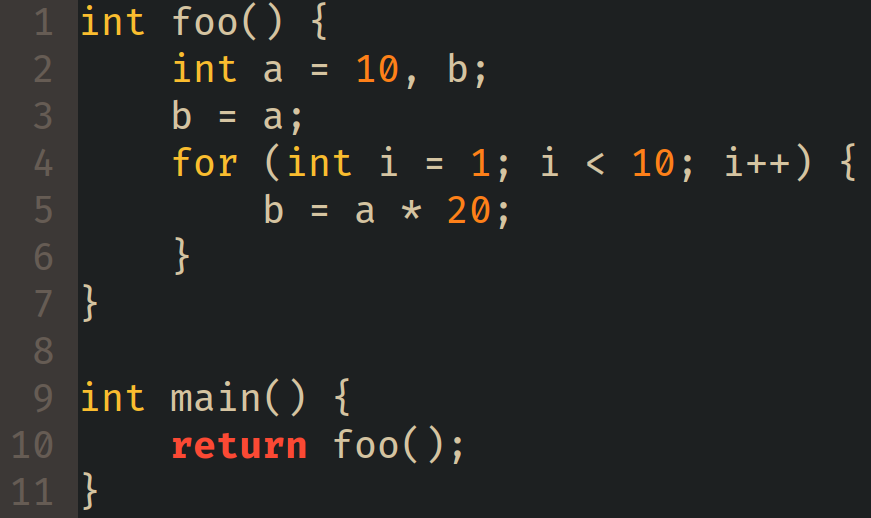
\includegraphics[width=0.90\columnwidth]{source.png}
        \caption{Example Loop Program}
        \label{fig:source}
    \end{figure}
\end{frame}
\begin{frame}
    \frametitle{Example of Data Depnedecy Graph}
    \begin{figure}
        \centering
        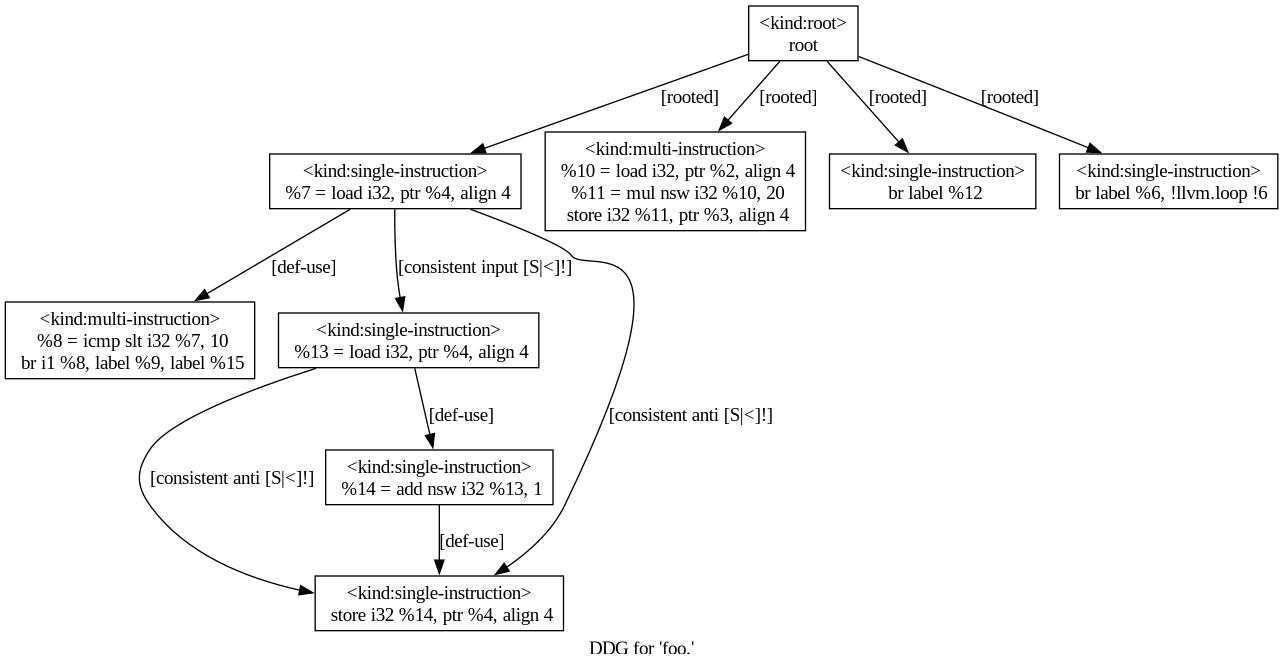
\includegraphics[width=0.90\columnwidth]{ddg.png}
        \caption{Example DDG for a Loop Program}
        \label{fig:ddg}
    \end{figure}
\end{frame}
\section{Online Assessment Timely Progress}
\begin{frame}
    \frametitle{Low-Overhead Online Assessment of Timely
    Progress as a System Commodity}
    \begin{itemize}
        \item The correctness of safety-critical systems depends on both their
            logical and temporal behavior. Control-flow integrity (CFI) is a
            well-established and understood technique to safeguard the logical
            flow of safety-critical applications. 
        \item This paper produces a milestone graph that is in turn checked
            by the the tracee to check for the timely progress of the system.
        \item Requires FPGA as the hardware for signal processing.
        \item ETM is used in the papers implementation.
    \end{itemize}
    \footnotetext{Chen, Weifan, et al. "Low-Overhead Online Assessment of
    Timely Progress as a System Commodity." 35th Euromicro Conference on
    Real-Time Systems (ECRTS 2023). Schloss Dagstuhl-Leibniz-Zentrum für
    Informatik, 2023.}
\end{frame}
\begin{frame}
    \frametitle{}
    \begin{figure}
        \centering
        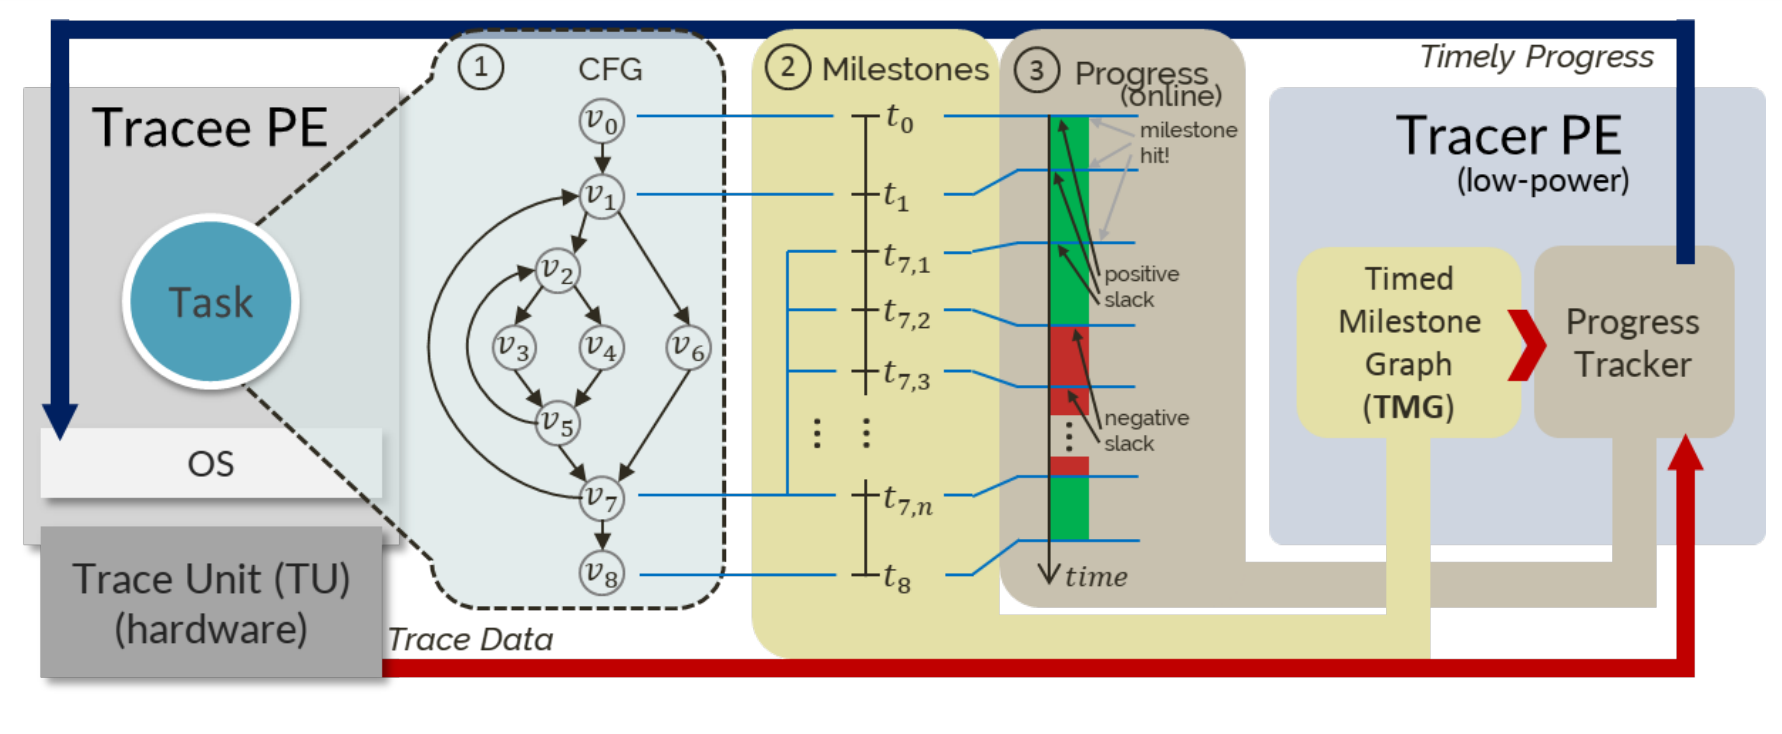
\includegraphics[width=1.0\columnwidth]{tp.png}
        \caption{High-level overview of the proposed system design, The CFG is
        used to produce the Timed Milestone Graph.}
        \label{fig:tp}
    \end{figure}
\end{frame}
\begin{frame}
  \centering \Large
  \emph{Thank You For Your Attention}
\end{frame}

\end{document}
